\iffalse
\documentclass[journal,10pt,twocolumn]{article}
\usepackage{graphicx, float}
\usepackage[margin=0.5in]{geometry}
\usepackage{amsmath, bm}
\usepackage{array}
\usepackage{booktabs}
\usepackage[utf8]{inputenc}
\usepackage{amsfonts}
\usepackage{amssymb}
\usepackage{graphicx}
\usepackage{multicol}
\usepackage{tabularx}
\usepackage{hyperref}
\usepackage{mathtools}
\DeclareUnicodeCharacter{2212}{-}
\providecommand{\norm}[1]{\left\lVert#1\right\rVert}
\providecommand{\abs}[1]{\left\vert#1\right\vert}
\let\vec\mathbf
\newcommand{\myvec}[1]{\ensuremath{\begin{pmatrix}#1\end{pmatrix}}}
\newcommand{\mydet}[1]{\ensuremath{\begin{vmatrix}#1\end{vmatrix}}}
\providecommand{\brak}[1]{\ensuremath{\left(#1\right)}}
\providecommand{\lbrak}[1]{\ensuremath{\left(#1\right.}}
\providecommand{\rbrak}[1]{\ensuremath{\left.#1\right)}}
\providecommand{\sbrak}[1]{\ensuremath{{}\left[#1\right]}}
%\providecommand{\norm}[1]{\left\lVert#1\right\rVert}
%\providecommand{\sbrak}[1]{\ensuremath{{}\left[#1\right]}}
%\providecommand{\lsbrak}[1]{\ensuremath{{}\left[#1\right.}}
%\providecommand{\rsbrak}[1]{\ensuremath{{}\left.#1\right]}}
%\providecommand{\brak}[1]{\ensuremath{\left(#1\right)}}
%\providecommand{\lbrak}[1]{\ensuremath{\left(#1\right.}}
%\providecommand{\rbrak}[1]{\ensuremath{\left.#1\right)}}
%\providecommand{\cbrak}[1]{\ensuremath{\left\{#1\right\}}}
%\providecommand{\lcbrak}[1]{\ensuremath{\left\{#1\right.}}
%\providecommand{\rcbrak}[1]{\ensuremath{\left.#1\right\}}}
%\newcommand{\myvec}[1]{\ensuremath{\begin{pmatrix}#1\end{pmatrix}}}
%\let\vec\mathbf

\title{\textbf{Optimization-Basic Assignment}}
\author{V.Meghana \hspace{9cm} FWC22045}
\date{October 2022}

\begin{document}

\maketitle
\paragraph{\textit{Problem Statement} -
\fi
Find the maximum value of $2x^3 – 24x + 107$ in the interval [1, 3]. Find the maximum value of the same function in [–3, –1].
\\
\solution
\iffalse
\section*{\large Solution}
\fi
    Using gradient ascent method,
\begin{align}
    x_n=x_{n-1}+\mu\frac{df(x)}{dx} \label{eq:12/6/5/109}
    \end{align}
    where
    \begin{align}
    \frac{df(x)}{dx}=6x^2-24 \label{eq:12/6/5/1010}
\end{align}
yielding
\begin{align}
    x_n=x_{n-1}+\mu(6x^2-24_{n-1})\label{eq:12/6/5/1011}
\end{align}
Choosing
\begin{align}
	x_0 &= 1, \mu = 0.001 \text{ and precision} = 0.00000001, 
	\\
	f_{max} &  \approx 139,
x_{max}   \approx -2.0
\end{align}
	\begin{figure}[!ht]
		\centering
		\includegraphics[width=\columnwidth]{12/6/5/10/figs/opt_basic.png}
		\caption{}
		\label{fig:12/6/5/10}
  	\end{figure}
\iffalse
\begin{align}
\end{align}
\end{enumerate}

\includegraphics[width=1\columnwidth]{opt_basic.png}
\centering \text{Graph of f(x) = $2x^3-24x+107$}

\end{document}
\fi
